\subsection{The Wave Equation}
The wave equation is a PDE that describes how waves, such as sound or electromagnetic waves, propagate through a medium by relating the second derivative of the wave function with respect to both time and position, illustrating the wave's behavior and propagation characteristics.

\subsubsection{Definition}
\noindent
Let us define a loop of string with the following assumptions:
\begin{itemize}
    \item The string is of length \(L\). A wave can travel through this medium at speed \(c\).
    \item The wave energy does not dissipate as it travels through the string.
    \item The initial wave propagation is defined as \(u(x,0) = f(x)\). Thus, the amplitude of the wave from the equilibrium position at position \(x\) at time \(t\) is \(u(x,t)\).
\end{itemize}

\noindent
Thus, the wave equation in one dimension is defined as follows \citep{Libretexts_2022b}:
\begin{equation} \label{eq:wave_equation}
    \frac{\partial^2 u}{\partial t^2} = c^2 \nabla^2 u = c^2 \frac{\partial^2 u}{\partial x^2}
\end{equation}

\noindent
Or in subscript notation,
\begin{equation} \label{eq:wave_equation_subscript}
    u_{tt} = c^2 u_{xx}
\end{equation}

\subsubsection{Application of the Fourier Transform}
Since \(u(x,t)\) is defined as the displacement of the wave at position \(x\) and time \(t\), we can apply the Fourier Transform to \(u(x,t)\) with respect to position \(x\) to reduce the \cref{eq:wave_equation_subscript} PDE into an ODE. Thus, let \(U(\kappa,t)\) be the Fourier Transform of \(u(x,t)\) with respect to \(x\).

\vspace{5mm}
\noindent
Taking the Fourier Transform of \cref{eq:wave_equation_subscript} with respect to \(x\),
\begin{equation}
    \mathcal{F}_x \left\{ u_{tt} \right\} = \mathcal{F}_x \left\{ \alpha^2 u_{xx} \right\}
\end{equation}

\noindent
Using \cref{fourier_scaling},
\begin{equation}
    \mathcal{F}_x \left\{ u_{tt} \right\} = \alpha^2 \mathcal{F}_x \left\{ u_{xx} \right\}
\end{equation}

\noindent
Using \cref{fourier_derivative},
\begin{align}
    \mathcal{F}_x \left\{ \frac{\partial^2 u(x, t)}{\partial x^2} \right\} & = i \kappa \mathcal{F}_x \left\{ \frac{\partial u(x, t)}{\partial x} \right\} \\
    & = -\kappa^2 \mathcal{F}_x \{ u(x, t) \} \\
    & = -\kappa^2 U
\end{align}

\noindent
Therefore,
\begin{align}
    \mathcal{F}_x \left\{ u_{tt} \right\} &= -\alpha^2 \kappa^2 U \\
    \frac{d^2 U}{dt^2} &= -c^2 \kappa^2 U \label{eq:wave_equation_fourier}
\end{align}

\subsubsection{Initial and Boundary Conditions}
\noindent
A hyperbolic secant distribution function will be used as the initial wave in the string for the ODE:
\begin{align}
    u(x, 0)=\sech(x) \label{eq:wave_equation_initial_condition}
\end{align}

\noindent
Though an open boundary condition could be employed, this would result in the wave propagating in one direction indefinitely. Instead of utilizing a large domain to represent this, the following periodic boundary condition will be employed such that the wave propagation travels out of the left of the domain and then feeds back into the right of the domain:
\begin{align}
    u(0, t) = u(L, t)
\end{align}

\subsubsection{Numerical Solution to Wave Equation}
\cref{eq:wave_equation_fourier} is a first-order ODE that can be easily numerically integrated. A numerical solution to \cref{eq:wave_equation_fourier} using a fifth-order Runge-Kutta approximation in Python is presented below. The Python code can be found in \cref{code:wave_equation}.

\begin{figure}[H]
    \centering
    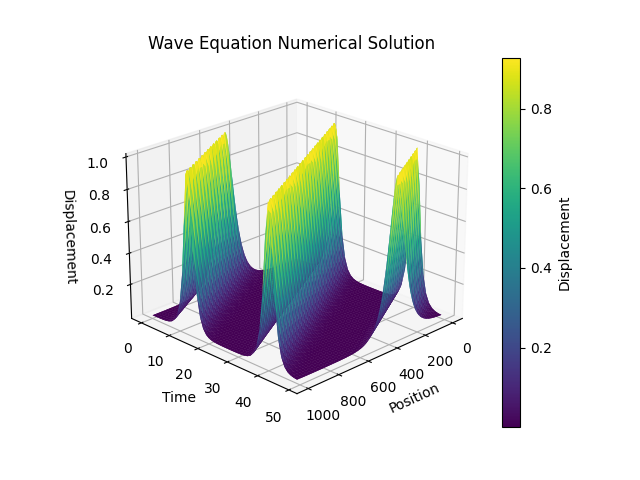
\includegraphics[width=100mm,height=\textheight,keepaspectratio]{images/wave_equation_numerical.png}
    \caption{Defining \cref{eq:wave_equation_initial_condition} the initial wave displacement, this plot shows the temperature change along \(x\) and \(t\) by performing a numerical integration of \cref{eq:wave_equation_fourier}.}
    \label{fig:wave_equation_numerical}
\end{figure}